\chapter[Introdução]{Introdução}

A agricultura familiar é um pilar fundamental da economia brasileira, sendo responsável pela produção de grande parte dos alimentos consumidos no Brasil, como feijão, arroz, mandioca, leite e verduras, garantindo emprego e renda para milhões de famílias. Além disso, a agricultura familiar também se destaca por ser uma alternativa produtiva mais sustentável que contribui para a preservação do meio ambiente, e é a principal fonte de produtos orgânicos.

Com o intuito de apoiar a agricultura familiar, em um \textit{Hackathon} da realizado no Campus Gama da UnB, surgiu a ideia do Agromart, que na  e posteriormente foi continuada ao longo de cinco projetos de conclusão de curso.

O Agromart consiste em uma aplicação que tem o objetivo de conectar agricultores e co-agricultores, para facilitar as relações comerciais de produtos oriundos da agricultura familiar. Tendo sua estrutura desenvolvida para ser compatível com o modelo de CSA, um modelo de agricultura sustentável que conecta consumidores e agricultores locais, em que os consumidores se comprometem a comprar uma cesta de alimentos periodicamente, e os agricultores se comprometem a fornecer alimentos frescos nesse período estabelecido.

\section{História do Agromart}

No ano de 2020 em um \textit{Hackathon} realizado no campus Gama  da UnB que tinha como tema: Cultivando Conexões, em que o objetivo era propor soluções tecnológicas que poderiam auxiliar a agricultura familiar, surgiu a ideia do Agromart. Inicialmente a proposta consistia em uma aplicativo mobile em que os produtores pudessem divulgar os seus pontos de venda, contendo informações sobre os produtos vendidos, preços, localização e meios para o contato, permitindo que através dessas informações disponibilizadas, os consumidores interessados pudessem ter acesso aos agricultores mais próximos, facilitando assim a relação entre as partes. \cite{rodriguesemacedo2021}

O projeto inicial conquistou o primeiro lugar do \textit{Hackathon}, então os alunos decidiram dar continuidade ao projeto através de um TCC no qual foi desenvolvido um novo aplicativo que incorporava o design do primeiro e buscava atender os novos requisitos levantados através de conversas com agricultores e professores. \cite{rodriguesemacedo2021}

O novo projeto tinha como ideia central o desenvolvimento de uma aplicação adequada ao modelo de parceria de uma CSA (Comunidade que Sustenta a Agricultura). Em uma CSA, se estabelece uma relação de produção e distribuição de produtos agroecológicos, em que o consumidor assume o papel de co-agricultor ao se comprometer por meio de uma assinatura a receber uma cesta de produtos previamente definidos pelo agricultor de forma periódica, com a possibilidade de adicionar outros produtos de acordo com a disponibilidade de cada um. Desse modo, o novo aplicativo proposto tinha como objetivo disponibilizar ao agricultor as seguintes funcionalidades: adição de novos produtos, definição da quantidade de cestas disponíveis, definição dos planos de assinaturas, e informações relativas à data, meio e local para realização da entrega ou coleta dos produtos. \cite{rodriguesemacedo2021}

Nos anos seguintes, o desenvolvimento do Agromart continuou por meio de quatro trabalhos de conclusão de curso. O primeiro trabalho realizado no ano 2021, foi desenvolvido com o objetivo de alterar a arquitetura do sistema para que cada CSA pudesse subir sua própria instância do Agromart, retirando assim a responsabilidade dos alunos e da faculdade pela manutenção dos servidores do aplicativo, mantendo apenas uma API dicionário em que seriam registrados os endereços de cada um dos servidores das CSA’s que subirem uma instância do Agromart.\cite{cellaefreitas2023} O segundo trabalho desenvolvido no ano de 2022, tinha como objetivo propor uma forma de pagamento dentro  do aplicativo, para facilitar as relações comerciais entre agricultor e co-agricultor. \cite{correiaeveludo2022}. Posteriormente, no ano de 2023 foi desenvolvido um trabalho com o objetivo de integrar o meio de pagamento dentro da aplicação do Agromart.\cite{augustiniebotinno2023} Ainda no ano de 2023, foi desenvolvido um trabalho que tinha como objetivo utilizar um serviço de Lambda na AWS para hospedar o servidor da API dicionário do Agromart, com o objetivo de reduzir os custos de hospedagem. \cite{ribeiroemagalhoes2023}

\section{Arquitetura e implementação do Agromart}
O Agromart é composto por três componentes principais: o aplicativo móvel, a API Dicionário e a API principal de cada CSA, como mostra a Fig. \ref{diagrama_arquitetura}. O funcionamento da aplicação consiste em uma API principal, administrada por cada CSA, que registra a URL do seu servidor na API Dicionário, que através do aplicativo móvel, possibilita o consumidor se conectar a uma das CSAs listadas na API Dicionário e interagir diretamente com ela.

O aplicativo móvel tem o objetivo de ser usado pelos clientes para realizar pedidos nas lojas da CSA escolhida. As tecnologias utilizadas no aplicativo móvel são: TypeScript, que é uma versão tipada da linguagem de programação JavaScript; React Native, um \textit{framework} para desenvolvimento mobile multiplataforma; e Expo, uma plataforma que simplifica o desenvolvimento de aplicativos usando React Native. Atualmente, o aplicativo está disponível apenas na versão Android, mas, por ter sido desenvolvido utilizando o React Native, que é uma ferramenta multi plataforma, é possível, futuramente, com poucas adaptações, disponibilizar uma versão iOS do aplicativo.

A API principal da CSA, tem o objetivo de salvar os dados dos produtos, planos, clientes e lojas de uma CSA. Cada CSA deve ter seu próprio servidor, desse modo, o Agromart é uma aplicação que funciona de forma decentralizada, sem qualquer interação entre os servidores de cada CSA. A API da CSA é feita na linguagem JavaScript, utilizando a ferramenta Strapi como Sistema Gerenciador de Conteúdo.
Além de ser consumida pelo aplicativo, a API principal também disponibiliza um painel de administração da CSA, onde é possível cadastrar produtos, visualizar pedidos entre outras funcionalidades.

A API Dicionário tem o objetivo de registrar as URLs de cada uma das CSAs que utilizam o Agromart, para que ao utilizar o App do Agroamrt, o usuário possa através dos endereços cadastrados na API Dicionário se conectar o servidor da CSA Desejada. A API Dicionário foi desenvolvida a linguagem JavaScript e o PostgreSQL como Sistema Gerenciador de Banco de Dados.

Anteriormente, existia um repositório web para os administradores das CSAs, mas, em trabalhos anteriores, esse painel foi arquivado, pois o painel de administrador disponibilizado pelo Strapi acessível através da API principal era uma forma mais eficiente de utilizar as funcionalidades de administrador da CSA.

\begin{figure}[h]
	\centering
	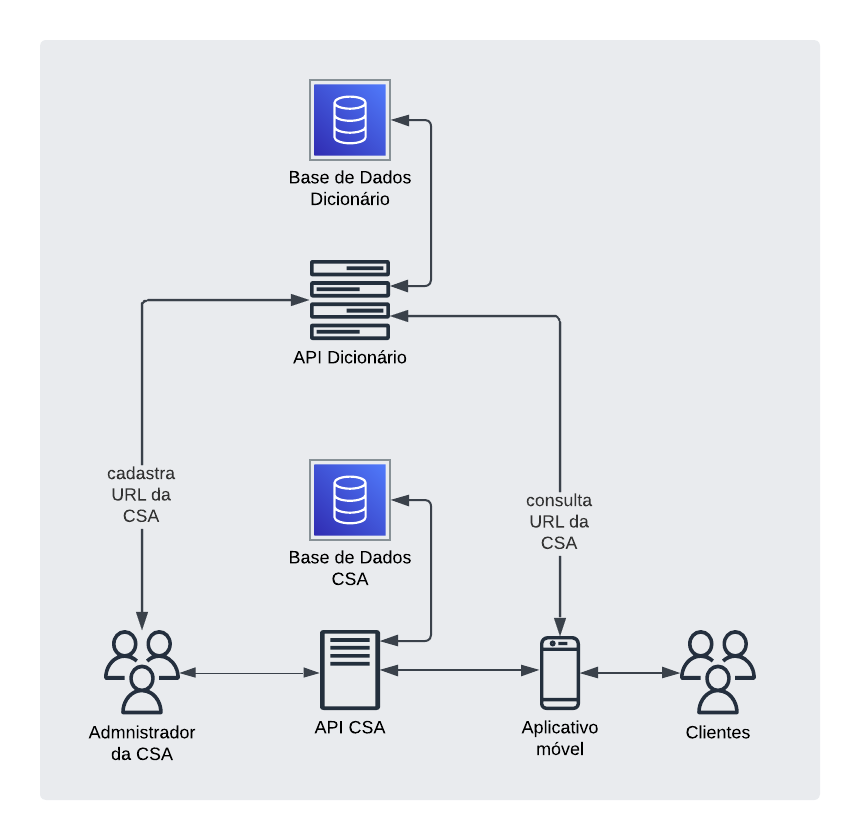
\includegraphics[keepaspectratio=true,scale=0.8]{figuras/diagrama_arquitetura.png}
	\caption{Diagrama de Arquitetura de Software Agromart}
	\label{diagrama_arquitetura}
\end{figure}

\section{Problema}
Desde 2020, quando a ideia do Agromart surgiu no \textit{Hackathon} que ocorreu na UnB-FGA, o projeto foi continuado ao longo de cinco trabalhos de conclusão de curso, tendo recebido contribuições de diversos alunos diferentes no desenvolvimento da aplicação. No entanto, esse desenvolvimento ocorreu sem seguir padrões claros para integrar as contribuições recebidas ao longo dos diferentes trabalhos realizados, o que comprometeu a organização do projeto como um todo.

A existência de diversos trabalhos que implementavam funcionalidades distintas mas não consideravam o Agromart como um todo, ao longo dos anos, comprometeu a unidade do projeto. Tal falta de unidade, pode-se notar através dos gráficos de \textit{branches} dos repositórios do servidor (Fig. \ref{agromart_api}) e do aplicativo mobile (Fig. \ref{agromart_app}), onde pode-se verificar a existência de várias \textit{branches} distintas que não foram unificadas no ramo principal de desenvolvimento. 

\begin{figure}[h]
	\centering
	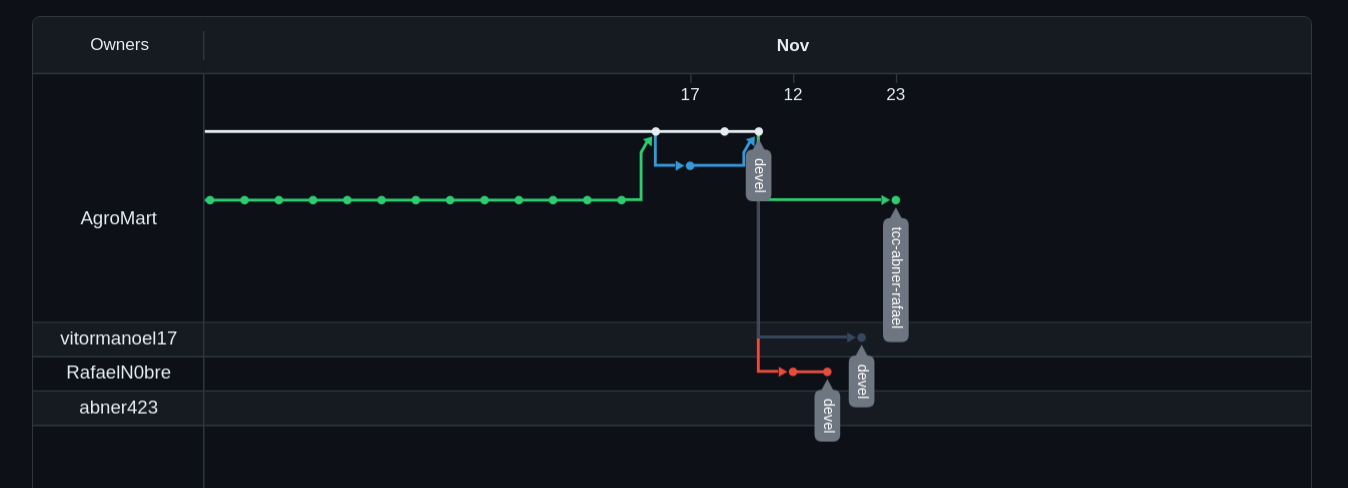
\includegraphics[keepaspectratio=true,scale=0.35]{figuras/agromart_api.png}
	\caption{Visualização gráfica das \textit{branches} da API Agromart}
	\label{agromart_api}
\end{figure}

\begin{figure}[h]
	\centering
	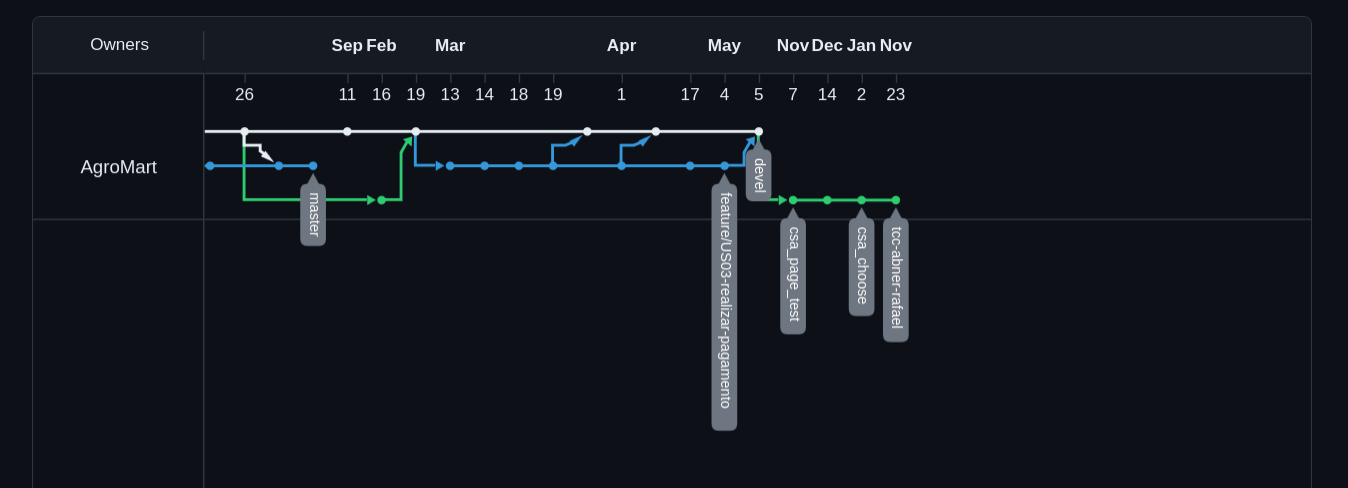
\includegraphics[keepaspectratio=true,scale=0.35]{figuras/agromart_app.png}
	\caption{Visualização gráfica das \textit{branches} do Aplicativo Mobile}
	\label{agromart_app}
\end{figure}

Além disso, a ausência de testes gerais feitos a cada nova implementação que garantisse o funcionamento da aplicação como um todo, tanto servidor quanto aplicativo mobile, causou incompatibilidades entre o aplicativo e o \textit{back-end}, comprometendo o funcionamento da aplicação. Um exemplo dessa incompatibilidade, é a ausência de modificações para se integrar o aplicativo mobile com a nova arquitetura do \textit{back-end}, implementada no trabalho \cite{cellaefreitas2023}, que utiliza uma API dicionário para listar as instâncias de CSAs que estão rodando o Agromart, para que o usuário selecione a instância desejada. Como consequência dessa incompatibilidade, a API dicionário não está sendo consultada pelo aplicativo na branch devel, e mesmo nas branches mais atualizadas, o aplicativo não está 100\% integrado com a arquitetura da API dicionário.

Desse modo, as inconsistências decorrente da falta de unidade do projeto como um todo, inviabilizam a publicação do aplicativo para download em lojas virtuais e a distribuição de uma versão do servidor do Agromart para que uma instância do servidor seja executada por uma CSA.

Outro efeito negativo de haver um sistema que não está totalmente integrado e em pleno funcionamento, é a inviabilidade de se receber contribuições externas no projeto, impossibilitando plena realização do carater \textit{open-source} da ideia original, que teria como possibilidade a recepção de contribuições para além da FGA, já que torna-se extremamente complicado contribuir para um sistema que apresenta erros de compilação ou em sua execução.

\section{Objetivo Geral}
Diante do exposto, surgiu a necessidade da realização de um trabalho que tenha como objetivo dar a unidade necessária para aplicação do Agromart, possibilitando que aplicativo móvel seja disponibilizado para download em lojas virtuais, que o Agromart possa ser utilizado por uma CSA, além de garantir que os futuros trabalhos tenham um ambiente mais propício para o desenvolvimento.

Este trabalho envolve a análise dos repositórios do Agromart em cada \textit{branch} existente, a realização de testes para detectar inconsistências nas funcionalidades do aplicativo móvel e da API principal, a correção de erros, defeitos e falhas para garantir o funcionamento adequado das funcionalidades básicas da aplicação, e a integração dos códigos de cada \textit{branch} em um novo marco zero dos repositórios do Agromart. Além disso, inclui a publicação do MVP (mínimo produto viável) do aplicativo móvel e do servidor para as CSAs, juntamente com uma documentação detalhada deste processo e outras atualizações de documentação das funcionalidades existentes e da arquitetura nos repositórios da API, do dicionário e do aplicativo móvel.

\section{Objetivo Específico}

\subsection{Unificação das \textit{Branches}}
Durante o desenvolvimento de software, é comum que diferentes versões do código sejam criadas em diferentes ramificações chamadas de "branches" para testar novas funcionalidades ou realizar correções sem afetar a versão principal do projeto. Neste objetivo, as diferentes \textit{branches} serão mescladas, formando uma nova versão unificada do projeto. Isso inclui o entendimento do conteúdo de cada \textit{branch} como também a resolução de conflitos de código que possam surgir durante a integração.

\subsection{Testes Funcionais Pós-Unificação}
Após a unificação do código, foi necessário realizar uma série de testes no aplicativo. Esses testes são fundamentais para verificar se todas as funcionalidades estão operando conforme esperado e se as correções realizadas surtiram o efeito desejado. A qualidade do software é beneficiada através destes testes.

\subsection{Correção de erros, falhas e defeitos}
Após a unificação das \textit{branches}, foi realizada a correção dos defeitos, erros e falhas identificadas no aplicativo móvel. O objetivo é garantir que o aplicativo opere de maneira estável e que os usuários possam utilizá-lo sem enfrentar problemas técnicos.

\subsection{Configuração do Ambiente}
A configuração do ambiente envolve preparar um espaço adequado onde o aplicativo possa ser desenvolvido e testado de forma eficaz. Isso inclui a configuração de servidores, bancos de dados e outros recursos necessários para garantir que a versão unificada do Agromart, possa ser desenvolvida e executada em um ambiente controlado.

\subsection{Publicação do Aplicativo na Play Store}
A Google Play Store é uma plataforma digital de distribuição de aplicativos para dispositivos Android. Publicar o aplicativo na Play Store significa disponibilizá-lo para que qualquer pessoa com um dispositivo Android possa baixá-lo e usá-lo. Esta etapa envolve não apenas a submissão do aplicativo para revisão pela Google, mas também garantir que ele esteja em conformidade com as políticas da plataforma e que sua versão publicada funcione corretamente.

\subsection{Atualização das Documentações}
Com a finalização das etapas anteriores, foi necessário atualizar as documentações do projeto para refletir as mudanças realizadas. Forma documentadas todas as funcionalidades existentes no aplicativo e na API principal, bem como uma explicação sucinta da arquitetura do sistema. Documentações atualizadas são essenciais para que outros desenvolvedores possam entender o estado atual do Agromart e contribuir com ele no futuro. Essas atualizações foram feitas no arquivo README de cada repositório.
